\section{Technique}
\label{sec:technique}

We model configurations as a set of key-value pairs, where
the keys are strings and the values have arbitrary type. This is
a common abstraction offered
by the POSIX system environment, the Java Properties API,
and the Windows registry.


\subsection{Overview}



%put to the profiling section?
%We also want to track caused effects of misconfigurations 

%For non-deterministic errors, \ourtool could potentially leverage one of
%several deterministic replay systems~\cite{Huang:2010:LLD}
%that can capture a buggy non-deterministic
%execution and faithfully reproduce it for late analysis.

Figure~\ref{fig:workflow} sketches the high-level workflow of our technique.
Our technique takes as input a Java program and its configuration options.
It first performs a propagation analysis to identify
the affected predicates for each configuration option (Section~\ref{sec:prop}).
Then, our technique \textit{selectively} instruments
the program only on those affected predicates. 
When diagnosing an error, users can run the failing inputs and
configurations on the instrumented program to obtain an execution
profile (Section~\ref{sec:profiling}).
Finally, our technique uses the obtained execution profile
to compare with the existing profiles in the pre-built database,
and diagnose the its root cause (Section~\ref{sec:analysis}).

The output error report is a ranked list
of suspicious configuration options that may cause the exhibited problem.

%, linking each configuration
%to its affected predicates

%\ourtool tracks dependencies introduced by both data and
%control flow. It propagates dependencies among xxx


\begin{figure*}[!]
  \centering
  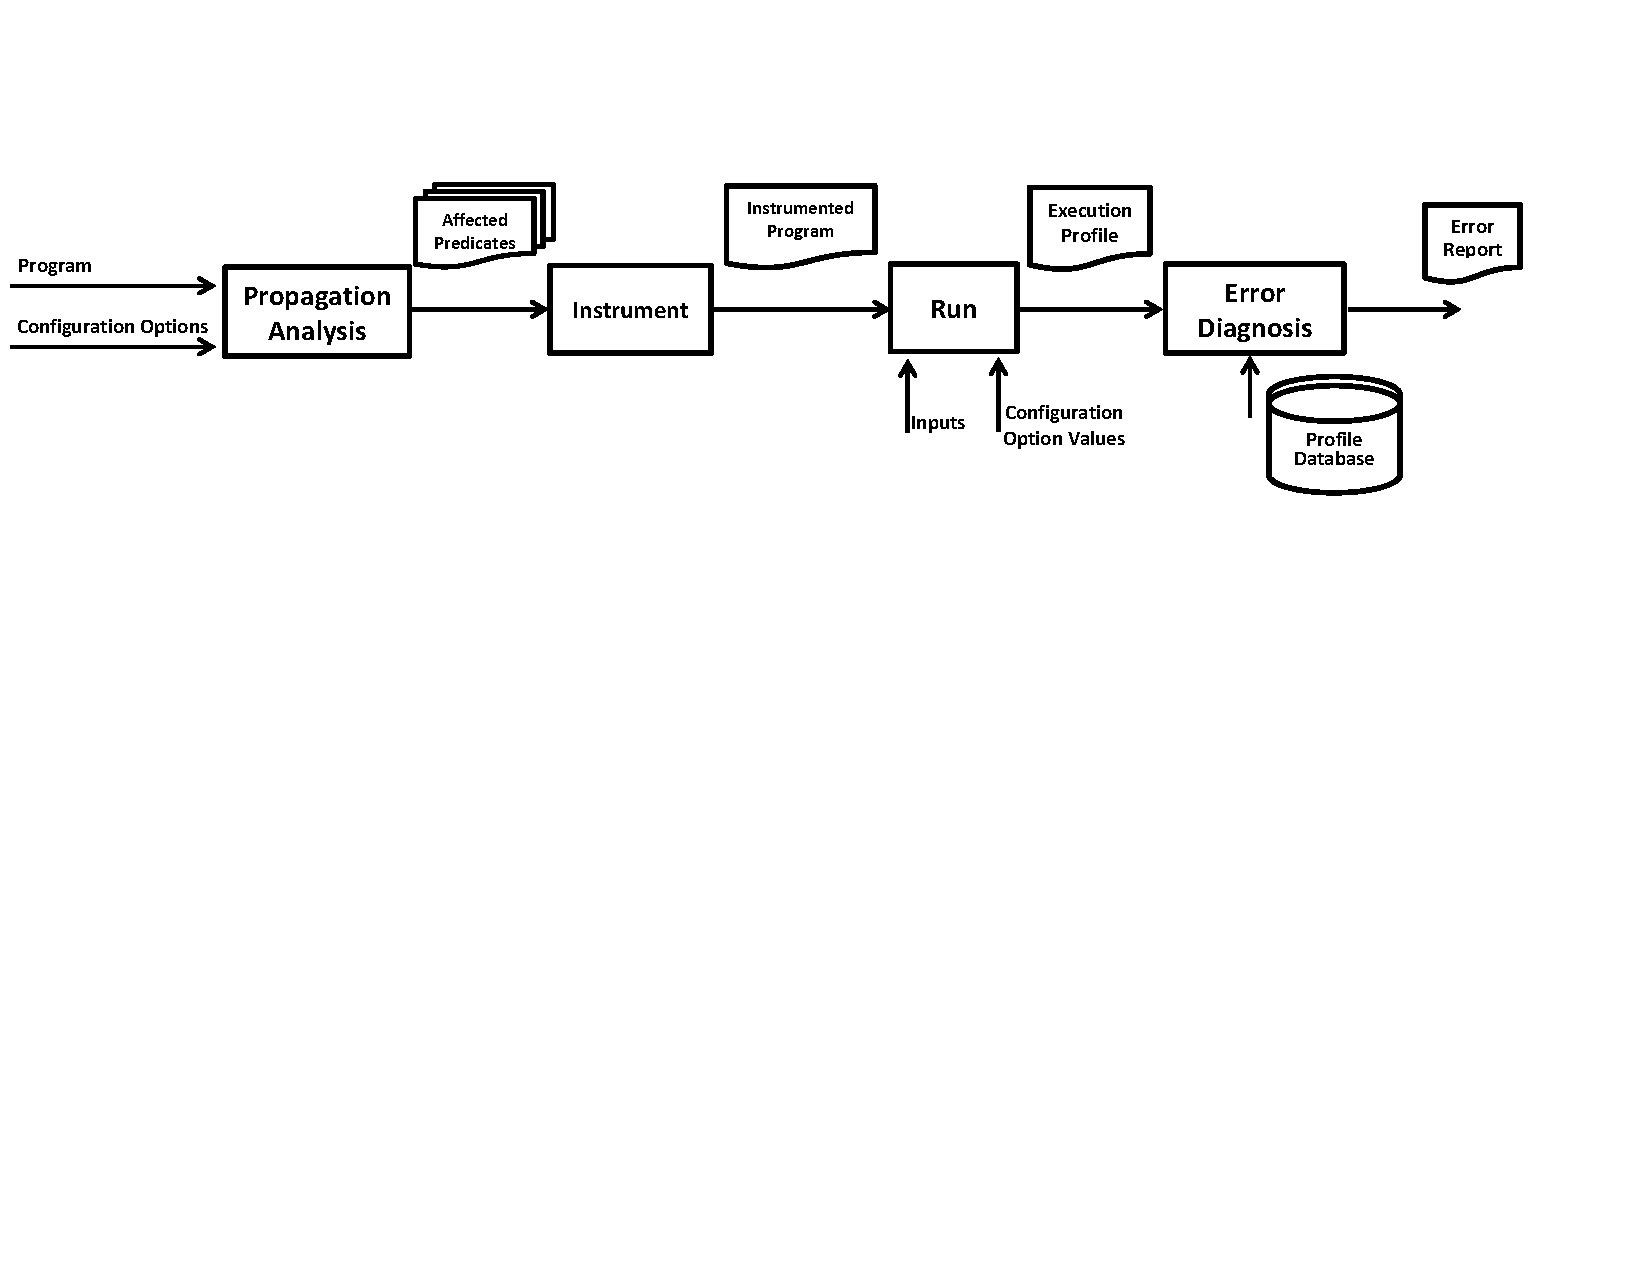
\includegraphics[scale=0.600]{architecture}
  \vspace*{-2.0ex}\caption {{\label{fig:workflow} The workflow of our configuration error diagnosis technique.
Phases ``Instrument'' and ``Run'' correspond to the Configuration Behavior Profiling step in Section~\ref{sec:profiling}.
The other two phases: ``Propagation Analysis'' and ``Deviation Analysis'' correspond to steps in Section~\ref{sec:prop} and Section~\ref{sec:analysis}, respectively.
}}
\end{figure*}

\subsection{Configuration Propagation Analysis}
\label{sec:prop}

For each configuration option, this step statically determines its affected program
fragments at the abstraction level of \textit{predicates}. Here, a \textit{predicate}
is a boolean expression in conditional or loop statements, whose evaluation result
decides to execute the followed statement or not. At runtime,
A predicate's outcome affects the program control flow and may alter
the consequent program state. In \ourtool, we focus on identifying and monitoring a program's
control flow instead of an arbitrary data flow for the following two
reasons: first, monitoring control flows
is essential since they propagate the majority of
configuration-related affects, while the value of a specific
data flow point can be largely input-specific;
and second, since the outcome of a program predicate can only be
either true or false, the number of recorded states resulting by monitoring
affected control flow is far less than monitoring possible  arbitrary
value changes in a program's data flow. In spite of that
predicate is not the only abstraction our technique could use,
we show empirically in Section~\ref{sec:evaluation} that choosing other
abstractions such as monitoring statement-level coverage information
or method-level invariant information yields less
diagnosis accuracy.


To identify predicates affectd by a configuration option, a straightforward
way is using program slicing~\cite{Horwitz:1988} to compute
a forward slice from the initialization statement of a
configuration option. Unfortunately, traditional slicing has
several limitations and can not be applied directly.
First, traditional slicing does not distinguish flows along
pointers from flows along values; thus, a resulting slice includes all statements that
\textit{may} affect a point of interest and often grows too large. Second,
in our context of configuration error diagnosis,
when having no knowledge of what inputs a software user would provide,
traditional slicing captures every single detail of the execution,
much of which may not be needed at all by pinpointing an incorrect
configuration option value.

Take the code in Figure~\ref{fig:example} as an example to illustrate
this problem.  The affected predicate set of 
configuration option \CodeIn{maxsize} computed by 
traditional slicing will include predicates in lines 104, 312, and 315.
However, the predicates in lines 104 and 315, though can be
affected by the value of \CodeIn{maxsize}, are incorrectly identified,
In other words, whether a sequence has an active flag (line 104) or
whether a sequence has been executed before (line 315)
is irrelevant with the value of \CodeIn{maxsize}. Monitoring
such predicates and linking their behaviors with the \CodeIn{maxsize}
option may introduce noise and decrease the diagnosis accuracy.

%However, if the provided input changes the workflow,
%instead of all data flow into it. 

To over this limitation, our technique uses thin
slicing~\cite{Sridharan:2007} as a manner to include
\textit{only} statements that are \textit{directly} affected by the configuration option.
Differing from traditional slicing, thin slicing
focuses on statements that flow values to the seed, ignoring the 
control flow dependencies as well as the uses of
base pointers. Essentially, thin slicing improves the relevance
of the slice by focusing on the statements that compute
and copy a value to the seed.
This property separates
pointer computations from the flow of configuration option value,
naturally connects a configuration option with its
directly affected statements, and makes thin slicing
especially attractive.

%A thin data dependence graph has exactly
%the same set of nodes as its corresponding data dependence
%graph. However, for an access \CodeIn{v.f}, the base pointer value
%in \CodeIn{v} is not considered to be used. 


We illustrate the advantages of using thin slicing 
by the same code excerpt in Figure~\ref{fig:example}.
A forward thin slice computed from \CodeIn{maxsize}
only includes the predicate in line 312.
In our experiments (Section~\ref{sec:evaluation}), 
we empirically compare traditional slicing with
thin slicing in diagnosing configuration errors, and show
that thin slicing is a better chioce.

%When Randoop is used to generate tests for different inputs (here,
%input mean programs under test), the created tests (method-call
%sequence at line 12) would be dramatically different.
%However, for similar inputs, the program execution flow should
%be similar.


%In fact, there is another configuration option $\blacksquare$
%that affect line 6.

% 

\subsection{Configuration Behavior Profiling}
\label{sec:profiling}

After identifying the affected predicates,
this step instruments the tested program offline,
inserting code to monitor the outcome of
each affected predicate at runtime, and associates it
with the affecting configuration option.


Take the code in Figure~\ref{fig:example} as an example,
the configuration option \CodeIn{maxsize} affects
the predicate at line 312. Thus, \ourtool inserts two instrumentation
statements before and after line 312 to keep the count of
the predicate being executed and the count of being evaluated to true,
as follows (the underlined parts):


\begin{CodeOut}
\begin{alltt}
310. private ExecutableSequence createNewUniqueSequence() \ttlcb
311.   Sequence newSequence = ...; 
       \underline{incrExecCount("maxsize", "newSequence.size() > maxsize");}
312.   if (newSequence.size() > maxsize) \ttlcb
         \underline{incrTrueCount("maxsize", "newSequence.size() > maxsize");}
314.     return null;
      ...
319. \ttrcb
\end{alltt}
\end{CodeOut}


The instrumented program summarizes an execution
as a vector of \textit{predicate profiles}.
Each predicate profile is a pair of configuration
option and one of its affected predicates.
The predicate profile also keeps the runtime
behavior of the affected predicate, including
the count of the predicate being executed and the count of it
being evaluated to true. 

\ourtool expresses an execution as
a predicate profile vector. As we
show in the experiments (Section~\ref{sec:evaluation}), such predicate profile
vectors, although by no mean complete, capture
sufficient information to permit users
to reason about the causal effects of configurations
and how they relate to a software's behavior, while
also imposing a moderate amount of performance impact
on foreground applications.


%health as the results of executing a set of predicates.

%As we will show in the experiments~\cite{}, this profile
%provides valuable information about the
%program execution and can help validate a test suite
%or indicate the usage context of a function
%or other computation.

%A software user seeking on specific piece of
%information or aiming to verify a specific invariant
%and uninterested in any other facts about the code
%may be able to use xxx to advantage, but will not
%get as much from it as a programmer open to other,
%possibly valuable information.


\subsection{Configuration Deviation Analysis}
\label{sec:analysis}

After obtaining a vector of predicate profiles from
an erroneous execution, \ourtool compares it with
existing traces from known correct executions, selects
similar traces for comparison (Section~\ref{sec:similar}),
identifies the most
behavioral-deviated predicates (Section~\ref{sec:deviation}), and then determines
its responsible options (Section~\ref{sec:linking}).


\subsubsection{Selecting Similar Traces for Comparison}
\label{sec:similar}

\ourtool's pre-built database contains a number of
traces from known correct executions. The traces
can be dramatically different from one another. To
better understand how and why the observed trace behaves
differently from the correct ones, \ourtool first
compares and contrasts the predicate profiles between
the erroneous execution and other correct ones, and
then selects a set of similar ones.

Given a trace $t$, \ourtool first aggregates
the observed predicate profiles, and creates a $n$-dimensional
vector $v_{t}$ =$\langle r_1, r_2, ..., r_n\rangle$ , where $n$
is the number of predicates in the program and each $r_i$ is
the ratio of the $i$-th predicate profile being evaluated
to true at runtime. If a predicate is not executed in
a particular execution, we assign \CodeIn{null} to its true ratio.


When comparing two traces $t_1$ and $t_2$, \ourtool computes
the inner-product distance of the normalized vectors, and treats
they are similar if the distance is below a threshold (default value: 0.3,
as we used in experiments). When computing the inner-product distance,
if the value of some dimensional is \CodeIn{null}. $\blacksquare$

For crashing errors, \ourtool does not perform this step in selecting
similar traces. Instead, it uses all available traces in the database
for comparison, because all traces in the database are correct, and can
be served as reference to identify the crashing root causes.

\subsubsection{Identifying Deviated Predicates}
\label{sec:deviation}


The comparison between an erroneous trace with a set
of \textit{similar} traces form a basis for our
automated error diagnosis approach. Given an erroneous trace and a set of similar but correct trace,
the differences in predicate profiles provide evidence for what parts of a program might be
incorrect and why. This helps to further reason about its root cause.


For each observed predicate $p$, \ourtool uses the following metric
to characterize its deviation degree in two traces $t_1$ and $t_2$.

\[
\|Deviation|(p) = |\phi(t_1) - \phi(t_2)|
\]

\[
\|\phi|(p) = \frac{2}{\frac{1}{\|trueRatio|(p)} + \frac{1}{totalNum(p)}}
\]

$trueRatio(p)$ is a function that returns the ratio of predicate $p$ being
evaluated to true in its observed executions, and $totalNum(p)$ is a function
that returns the total number of observations of predicate $p$.

The metric $\phi$ has some good properties in characterizing the $\blacksquare$

For non-crashing errors, since the obtained trace is a complete one,
\ourtool computes the $Deviation$ metric for each observed predicate in
both traces, and ranks predicates decreasingly based on the computed value.

For crashing erros, since the obtained trace is incomplete,
\ourtool computes the $Deviation$ metric for the predicates only appearing
in the crashing trace, and ranks them decreasingly based on the computed value.


%\subsubsection{Filtering Execution Noises}
%remove some off-by-one


\subsubsection{Linking Predicates to Root Causes}
\label{sec:linking}

The last step in \ourtool is to link those behavioral-deviated
predicates to its root causes, and rank the suspicious
configuration options as the output.

The intuition behind is that \ourtool determines that
altering a configuration option may change the application�s
control flow such that it deviates from the correct trace,
 it reports that option as a possible root cause.

When comparing an erroneous trace with a set of correc traces,
\ourtool first ranks suspicious configuration options between
each trace pair, and then averages the ranking across traces.

It first identifies the most deviated predicate profile, and
its affecting predicate.
It identifies the configuration option
affecting the highest ranked predicate profile as the most likely
root cause; in the case of ties, it ranks all tied options
based on its distance in a thin slicing SDG.
%as being equally likely to be the root cause.

Finally, needs to average the results


\subsection{Discussions}

We next some design issues in \ourtool.

\vspace{1mm}
\noindent \textbf{Differences between program inputs and configuration options.}

The fundamental differences between inputs and options. A configuration
option is fixed before input.

Configuration customize the overall program behavior, when inputs is a specific

\vspace{1mm}
\noindent \textbf{Why cannot use unit test executions?}
Why cannot use unit test to achieve the trace? since it is incomplete


%why cannot delta debugging? no working state, no predicate

\vspace{1mm}
\noindent \textbf{Why not only store correct traces in the database?}

why not store failed traces in the database? (developers
cannot anticipate the error behaviors). A broader question is which
informatin should be stored in the database for comparison, now, we use
profiling info, what about statement info? invariant? they all
summarize valuable info.

%Why dynamic slicing is not usable? No seed statement, and great overhead. Using JSlicer incurs
%a great overhead. It needs to track every instruction and
%perform synchronization when dependence graph is updated.

%Our technique can be seen as a way to reduce overhead,
%including selective profiling, and static pre-processing
%techniques.

